\begin{explanationbox}
\textbf{\textcolor{CExplanation}{一句话直觉}}

连不等式 $N < f(x) < M$ 可通过多种代数形式等价表达，每种形式在不同解题场景下有独特优势。

\medskip
\textbf{\textcolor{CExplanation}{核心拆解}}
\begin{description}[style=nextline, leftmargin=2.8em, labelsep=0.5em, itemsep=0.45em]
    \item[\textbf{要点一（等价性）：}] 五个命题互为充分必要条件，从任一形式可推出其他形式。
    \item[\textbf{要点二（变形技巧）：}] 通过移项、通分、平方等代数操作，实现形式间的转换。
    \item[\textbf{要点三（条件注意）：}] 倒数形式需保证 $f(x)-N > 0$，该正值条件也可由倒数不等式本身推出；取倒数前须确认两数同号。
\end{description}

\medskip
\textbf{\textcolor{CExplanation}{几何本质（数轴位置）}}

在数轴上，点 $N$ 和 $M$ 确定一个开区间 $(N, M)$。函数值 $f(x)$ 位于该区间内等价于 $f(x)$ 到区间中点 $\frac{M+N}{2}$ 的距离小于区间半长 $\frac{M-N}{2}$。

\medskip
\textbf{\textcolor{CExplanation}{代数意义（符号分析）}}

乘积形式 $(f(x)-M)(f(x)-N) < 0$ 表明 $f(x)-M$ 与 $f(x)-N$ 异号，即 $f(x)$ 介于 $M$ 和 $N$ 之间。分式形式 $\frac{f(x)-N}{M-f(x)} > 0$ 表明分子分母同号，又因分子分母之和为 $M-N>0$，两者必同时为正。倒数形式利用函数 $\frac{1}{t}$ 在 $t>0$ 时的单调递减性。

\medskip
\textbf{\textcolor{CExplanation}{考点价值（不等式转化）}}
\begin{itemize}[leftmargin=*, itemsep=0.5em, topsep=0.4em]
    \item \textbf{考法一（证明等价）：} 在证明题中，需证 $N < f(x) < M$，可转化为证明乘积形式或绝对值形式，有时更易操作。
    \item \textbf{考法二（求解范围）：} 当不等式包含参数或需解 $x$ 时，转化为分式形式或倒数形式可能简化计算。
\end{itemize}

\medskip
\textbf{\textcolor{CExplanation}{顿悟点}}

无论形式如何变化，实质都是表达 $f(x)$ 落在开区间 $(N, M)$ 内。选择哪种形式取决于当前问题的最简路径。

\medskip
\textbf{\textcolor{CExplanation}{使用场景}}
\begin{itemize}[leftmargin=*, itemsep=0.5em, topsep=0.4em]
    \item \textbf{场景一（证明题）：} 需要证明函数值满足连不等式时，优先考虑乘积形式或绝对值形式进行变形。
    \item \textbf{场景二（求解题）：} 给定连不等式求自变量的取值范围时，可尝试分式形式或倒数形式分离变量。
\end{itemize}
\medskip
\textbf{三个数轴图解（令 $t=f(x)$）}
\begin{center}
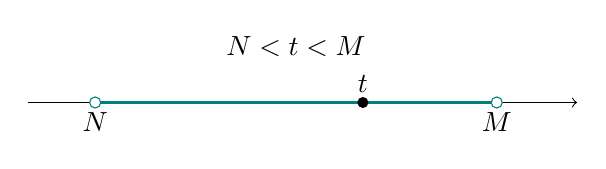
\begin{tikzpicture}[x=0.85cm,y=0.7cm]
\draw[->] (-1,0)--(7.2,0);
\draw[very thick,teal] (0,0)--(6,0);
\draw[teal,fill=white] (0,0) circle(2pt) (6,0) circle(2pt);
\fill (4,0) circle(2pt);
\node[below] at (0,0){$N$};\node[below] at (6,0){$M$};\node[above] at (4,0){$t$};
\node[above] at (3,0.65){$N<t<M$};
\end{tikzpicture}

\begin{tikzpicture}[x=0.85cm,y=0.7cm]
\draw[->] (-2,0)--(8,0);
\draw[very thick,teal] (0,0)--(6,0);
\draw[fill=white] (0,0) circle(2pt) (6,0) circle(2pt);
\node[below] at (0,0){$N$};\node[below] at (6,0){$M$};
\node[above] at (-1,0){$+$};\node[above,teal] at (3,0){$-$};\node[above] at (7,0){$+$};
\node at (3,1){$(t-M)(t-N)$ 的符号};
\end{tikzpicture}

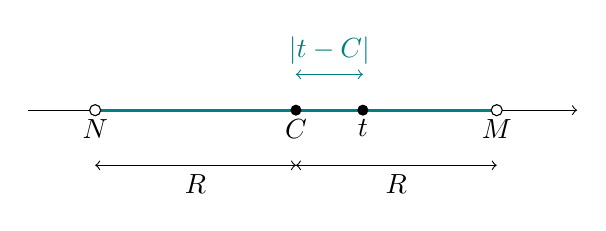
\begin{tikzpicture}[x=0.85cm,y=0.7cm]
\draw[->] (-1,0)--(7.2,0);
\draw[very thick,teal] (0,0)--(6,0);
\draw[fill=white] (0,0) circle(2pt) (6,0) circle(2pt);
\fill (3,0) circle(2pt) (4,0) circle(2pt);
\node[below] at (0,0){$N$};\node[below] at (3,0){$C$};\node[below] at (6,0){$M$};\node[below] at (4,0){$t$};
\draw[<->] (0,-1)--node[below]{$R$}(3,-1);
\draw[<->] (3,-1)--node[below]{$R$}(6,-1);
\draw[<->,teal] (3,0.65)--node[above]{$|t-C|$}(4,0.65);
\end{tikzpicture}
\end{center}
\textbf{如何选择：} 已有两个因式时用乘积；已有平方或对称距离时用绝对值；已有端点差的比值时用分式；已有倒数比较时用倒数。若原式直接移项最短，就不必变形。
\end{explanationbox}
